\section{Voraussetzungen}

\subsection{Versuchsziel}

Im Fortgeschrittenen-Praktikum „Quantenkryptographie“ besteht das Versuchsziel
darin, einen digitalen Schlüssel unter Verwendung des BB84-Protokolls
quantenkryptographisch verschlüsselt über eine kurze Distanz zu übertragen.
Die hierfür benötigten quantenmechanischen Zustände werden durch verschiedene
Polarisationen des zur Übertragung verwendeten Laserlichts repräsentiert.

\subsection{Motivation}

Um vertrauliche Informationen auszutauschen, ist die Verschlüsselung das
Mittel der Wahl. Der Sender wird allgemeinhin mit Alice, der Empfänger mit Bob
bezeichnet. Werden während der Überbringung oder Übertragung die Daten von
einem Dritten, der Konvention nach Eve genannt, abgefangen beziehungsweise
mitgelesen, so erhält dieser nicht ohne weiteres Aufschluss über die Informationen.
Die gesicherte Kommunikation ist also nur so lange gewährleistet, wie die zur
Verschlüsselung verwendeten Parameter (der Schlüssel) nur Alice und Bob bekannt
sind. Die Herausforderung verschiebt sich nun von der abhörsicheren
Informationsübermittlung hin zur Frage, wie der Schlüssel ausgetauscht werden
kann.

Bei der asymmetrischen Verschlüsselung wird der Schlüssel in einen privaten und
einen öffentlichen Schlüssel geteilt. Durch die Verwendung von Einmal-Funktionen
entfällt nun die Notwendigkeit einer Schlüsselübergabe. Allerdings kann eine
unbefugte Entschlüsselung nicht prinzipiell ausgeschlossen werden. Man hofft,
dass eine kurzfristige Entschlüsselung auf Grund des hohen Aufwandes nicht möglich
ist. Mit steigender Leistungsfähigkeit der Computer sinkt somit die Sicherheit
der heute verwendeten asymmetrischen Verschlüsselungssysteme, wodurch die Forschung
nach alternativen Lösungsansätzen an Bedeutung gewinnt.

Die symmetrische Verschlüsselung erfordert einen Schlüsselaustausch vor der
Informationsübertragung. Wenn der Schlüssel ebensolang wie die zu verschlüsselnde
Information ist, so ist es prinzipiell unmöglich aus den verschlüsselten Daten
etwas zurückzugewinnen. Man spricht in diesem Fall von dem One-Time-Pad. Gelingt
es allerdings Eve Kenntniss über den Schlüssel zu gewinnen, so ist eine sichere
Verschlüsselung nicht mehr gewährleistet.

Die klassische Kryptographie sieht sich also mit zwei Problemen konfrontiert:
\begin{enumerate}[a)]
 \item Wie kann ein nicht-deterministischer Schlüssel erzeugt werden?
 \item Wie kann ausgeschlossen werden, dass der Schlüssel abgehört wurde?
\end{enumerate}

Die Quantenkryptographie erlaubt die Lösung dieser beiden Probleme. Durch
den der Quantenmechanik eigenen intrinsischen Zufall ist das Vorhersagen
des aus quantenmechanischen Zuständen abgeleiteten Schlüssels nicht möglich.

Außerdem folgt aus dem No-Clone-Theorem, dass der Schlüssel nicht unbemerkt
abgehört werden kann. Hierfür ist es allerdings notwendig, für das Übetragen des
Schlüssels jeweis nur ein Teilchen zu benutzen um einen quantenmechanischen
Zustand zu übertragen.

Nachdem der Schlüssel übertragen wurde und ein Abhören nicht stattgefunden hat,
kann nun auf einem öffentlichen Kanal die chiffrierte Nachricht übermittelt werden.
Für jeden, der nicht im Besitz des Schlüssels ist, ist die verschlüsselte
Botschaft nicht lesbar und daher nutzlos.

\subsection{Physikalische Grundlagen}

Die quantenkryptographische Sicherheit kann mit Hilfe des BB84-Protokolls
erreicht werden. Hier wird die Polarisationsrichtung von Photonen verwendet, um
Informationen zu übertragen. Zunächst erzeugt Alice unpolarisierte Photonen mit
Einzelphotonenquellen wie beispielsweise Quantenpunkten. Diese werden durch
einen Polarisationsfilter geleitet, der die Photonen linear polarisiert. Die
Richtung dieses Filters kann dabei in \SI{45}{\degree}-Schritten von 0 bis
\SI{135}{\degree} eingestellt werden. Dabei stellen die Positionen bei null und
\SI{90}{\degree} die Achsen eines „ungedrehten“, rechtwinkligen
Koordinatensystems dar, während die Einstellung bei 45 und \SI{135}{\degree} die
Achsen eines gedrehten, ebenfalls rechtwinkligen Koordinatensystems darstellen.
Die beiden Koordinatensysteme repräsentieren jeweils eine Basis, bezüglich der
die Polarisation der Photonen gemessen wird. Die konkrete Wahl der Basis von
Alice wird zufällig eingestellt. Die polarisierten Photonen werden nun zu Bob
geleitet, der das Licht ebenfalls mit einem Polarisationsfilter analysiert. Die
Wahl der Basis von Bob erfolgt zufällig. Schließlich können die Photonen, die
den Filter passiert haben, mit einem Detektor nachgewiesen werden.

Um aus den Messungen der Photonen einen Schlüssel zu erzeugen, vergleichen
Alice und Bob die Wahlen ihrer Basen. Nur wenn beide zufällig die gleichen Basen
gewählt haben, werden die in diesen Fällen gemessenen Werte weiter verwendet, da
nur hier die Messergebnisse von Bob deterministisch sind und somit Informationen
liefern können. Schließlich müssen sie sich einigen, welche der Achsen der
beiden Basen von Alice einer Null bzw. einer Eins entsprechen. So können beide
nur über den Vergleich der verwendeten Basis und insbesondere ohne den
Vergleich der Messwerte einen Schlüssel konstruieren.

Wenn Eve versuchen würde, die Polarisation der von Alice gesendeten Photonen zu
messen und ein Photon gleicher Polarisation zu Bob zu senden, würde dies
dadurch auffallen, dass Eve statistisch gesehen in der Hälfte der Fälle die
falsche Basis gewählt hat und in diesen Fällen rein zufällige Messungen macht
und daher in \SI{50}{\percent} der Fälle falsch polarisiertes Licht zu Bob
schickt. Alice und Bob können beispielsweise einen Teil ihres Schlüssels
veröffentlichen und vergleichen, wie oft sie unterschiedliche Ergebnisse
produziert haben, was geschehen würde, wenn Eve eine andere Basis als Alice und
Bob gewählt hat. Wenn dies häufig der Fall ist, bedeutet dies, dass ihre
Transaktion abgehört wurde. 

\subsection{Versuchsaufbau}

Der für den Versuch konkret verwendete Aufbau weicht in einigen Details vom
prinzipiellen Schema ab. Zunächst wurde keine wirkliche Ein-Photonen-Quelle
verwendet, sondern ein Laser, dessen Intesität so stark abgeschwächt wurde,
dass es sehr unwahrscheinlich ist, dass mehr als ein Photon gleichzeitig
emittiert wird.

Weiterhin wurden die Photonen durch einen Strahlteiler geleitet, der nur
vertikal porarisiertes Licht passieren lässt und die vertikalen Anteile aus der
Apparatur herausführt. In einem nächsten Schritt passieren die Photonen einen 
„elektro-optischen Modulator“ (EOM), wie sie in \fref{aufbau} zu sehen sind.

\begin{figure*}[htb]
 \centering
 \includegraphics[page=8,viewport=166 482 445 565,clip,%
  width=0.8\paperwidth,keepaspectratio]{%
  ../doc/crypto3}
 \caption{Aufbau des Experiments}
 \label{fig:aufbau}
\end{figure*}

Dabei handelt es sich um Geräte, die den Lichtstrahl, der durch sie
hindurchläuft, durch ein doppelbrechendes Medium leiten, dessen
Brechungsindizes von der angelegten elektrischen Spannung abhängen. Man kann
über eine Software diesen Spannungswert variieren und somit das optische
Verhalten des doppelbrechenden Kristalls beeinflussen. Da die Wellenlänge der
Photonen konstant und bekannt ist (ca. \SI{633}{nm}), kann gezielt eingestellt
werden, ob sich die EOMs wie $λ/4$- oder $λ/2$-Plättchen verhalten. Im
Endeffekt resultieren je nach gewähltem Spannungswert horizontal, vertikal oder
rechts- bzw. links-zirkular polarisierte Photonen, die zu Bob gesendet werden.
Ein Nachweis, dass zirkular polarisiertes Licht für unsere Zwecke geeignet ist,
wird in \textcolor{red}{\sref{zirkular}} geführt.

Auf der Seite von Bob wird das eintreffende Licht zunächst durch einen weiteren
EOM geleitet. Hier wird die Polarisationsrichtung des Lichts erneut um einen
gewissen Winkel gedreht, der mit einer Spannung geregelt werden kann.
Anschließend wird der Lichtstrahl erneut durch einen Strahlteiler geleitet, der
nur die vertikal polarisierten Anteile passieren lässt. Schließlich werden die
Photonen mit einer Avalanche-Photodiode (APD) registriert.
